%======================================================================
\section{Two dimensions: the training distribution decides}
\label{sec:results2d}
%======================================================================

In 1D a model trained on whole periodic domains transfers. In 2D the same
approach fails, and the cause is not the architecture but the data the
model is trained on. This section shows the failure, the fix, the
canonical recipe that results, and how well the transferred models
reproduce the scaling of $\DKY$ with domain size. All errors are relative
to the references of Table~\ref{tab:truth}; for Kolmogorov flow at
$\alpha=0.05$, $1\times$, each model run is scored against the truth from
its own initial condition (Sec.~\ref{sec:truth_uncertainty}).

%----------------------------------------------------------------------
\subsection{Training on a small periodic box fails, and coupling makes it worse}
\label{sec:box_vs_window}
%----------------------------------------------------------------------

Our first 2D models were trained, like the 1D model, on whole periodic
domains: an $8\times8$-site box for both systems. Both reproduce the
dimension of their training box tolerably (2D KS: $13.7\%$ error;
Kolmogorov flow at $\alpha=0.05$: $3.7\%$). Under transfer they degrade
(Fig.~\ref{fig:box_vs_window}). The 2D KS model is $23\%$ low at $66^2$,
consistently across three initial conditions. At $\alpha=0.05$ the
Kolmogorov model is $38\%$ low at $2\times$; at $\alpha=0.1$ it is
accurate at $2\times$ ($1.9\%$) but $15\%$ low at $3\times$ and $23\%$ low at
its own size.

The propagator of these models reaches 6 sites per step on an 8-site
periodic ring, so it sees $75\%$ of its training domain and can use the
periodic wrap-around, a self-interaction that a larger domain does not
have. The local statistics of a small box also differ from the local
statistics inside a large domain wherever the flow is not exactly
extensive. A model fitted to the box therefore learns the wrong local
rule for the domain it is deployed on.

A natural response is to give the model more non-local information. We
tried three versions, each trained on the same box: the exact
Biot--Savart velocity as an additional input (D2), a learned coarse
``regional'' scale with its own mixer (D3), and a box-trained model with
the exact velocity input (C9). All three train to low loss at the box
size, and all three collapse under transfer: $\DKY$ falls to between 0
and 5 at $2\times$ and $3\times$, errors of $93$--$100\%$
(Fig.~\ref{fig:box_vs_window}(c)). Each new coupling path is trained only
on inputs from one small periodic domain and meets wavenumbers,
amplitudes and aggregation patterns at deployment that it never saw.
More expressive coupling made transfer worse, not better.

%----------------------------------------------------------------------
\subsection{Training on windows of a large domain fixes it}
\label{sec:window_fix}
%----------------------------------------------------------------------

We kept the architecture and changed only the data: one large domain
($6\times44$ per side for 2D KS, $16\times2\pi$ wide for Kolmogorov
flow), trained on crops with forced halos (Sec.~\ref{sec:crop_training}).
For 2D KS the crops are cut in both directions, so no training sample
contains a whole periodic direction. The effect is large
(Fig.~\ref{fig:box_vs_window}):
\begin{itemize}
\item 2D KS: $13.7\%\to0.9\%$ at $44^2$ and $23\%\to3.9\%$ at $66^2$.
\item Kolmogorov, $\alpha=0.05$: $37.8\%\to7.4\%$ at $2\times$, and $6.3\%$ at
  $3\times$, a size at which no box-trained model was evaluated.
\item Kolmogorov, $\alpha=0.1$: $15.1\%\to4.0\%$ at $3\times$ and
  $23.4\%\to8.6\%$ at $1\times$, but $1.9\%\to18.8\%$ at $2\times$.
\end{itemize}
The one regression, $\alpha=0.1$ at $2\times$, is the box model's
best size; the window-trained model over-predicts there by $15$--$23\%$
across initial conditions. The window-trained models never see a $2\pi$
periodic box, yet they reproduce the dimension of that box to within
about $9\%$ at both drags.

%----------------------------------------------------------------------
\subsection{The canonical recipe}
\label{sec:canonical_results}
%----------------------------------------------------------------------

Two further changes produced the recipe of Sec.~\ref{sec:canonical_recipe}.

\para{A per-patch autoencoder.} Training on crops loses a margin of
$\Renc+\Rdec$ sites at every crop edge. A per-patch autoencoder has no
reach and no margin; with more channels it loses no accuracy, at the
price of a reconstruction error about $30\%$ higher (2D KS). At
$\alpha=0.05$ and equal training data, a per-patch autoencoder with
$c=6$ gives $8.9\%$, $7.7\%$ and $3.0\%$ error at $1\times$, $2\times$ and
$3\times$ (three initial conditions), against $7.3\%$, $7.4\%$ and $6.3\%$
for the full-reach $c=3$ model; a second training seed gives $7.6\%$,
$0.2\%$ and $3.0\%$. Removing only the decoder's reach at $c=3$ gives
$5.0\%$, $9.3\%$ and $13.3\%$ (one initial condition), with the error
growing with size: three channels cannot hold a $16\times16$ patch's
chaotic content without borrowing from neighbours, six can. At equal
$c=6$, a full-reach control is worse at $1\times$ ($15.3\%$), better at
$2\times$ ($4.5\%$) and similar at $3\times$ ($4.5\%$), from one initial
condition (Fig.~\ref{fig:appendix_panels}(b)). The per-patch
design is therefore at least as accurate, needs no crop margin, and, as
Sec.~\ref{sec:da_results} shows, makes the latent observation operator
exactly local.

\para{Rollout length.} Short rollouts in training can leave the
free-running model under-constrained (Sec.~\ref{sec:fail_regimes}), and
long ones bias $\DKY$ downward (Sec.~\ref{sec:fail_mse}). The models
reported here use $\kmax=32$ for 2D KS and for Kolmogorov flow at
$\alpha=0.025$, $\kmax=16$ at $\alpha=0.1$, and the original $\kmax=12$ at
$\alpha=0.05$; at that drag a $\kmax=32$ model trained otherwise identically
(\texttt{k\_xs005\_noreg} in Appendix~\ref{app:tables}) gives
comparable errors ($6.2\%$, $5.2\%$, $7.2\%$).

\para{Selecting a model without the truth.} At $\alpha=0.1$ we trained six
variants that differ in $\kmax$ ($16$--$32$) and in the autoencoder's
regularizers (Sec.~\ref{sec:fail_mse}). Their errors against the truth
trade off between sizes, so choosing the one with the smallest error at
one size would select on the reference itself. We instead fixed a rule
before evaluating it (Appendix~\ref{app:architecture}): a variant is
eligible if its free rollouts reproduce the training data's vorticity
variance and forcing-band energy share to within $15\%$ at every size,
and among eligible variants the one with the lowest physical-space
forecast error, eight steps ahead on the held-out validation trajectory,
is selected. All six are eligible (largest deviation $6.3\%$); the
selected model's forecast error is lower than every other variant's by
at least 4.6 paired standard errors. Its errors against the truth are
$0.9\%$, $5.9\%$ and $2.6\%$ at $1\times$, $2\times$ and $3\times$; the
variant previously chosen for its $3\times$ accuracy gives $8.8\%$,
$9.9\%$ and $2.9\%$.

\para{Results.} Table~\ref{tab:transfer2d} collects the canonical
models. For 2D KS the error is $2.0\%$ at the native size and $0.6\%$ at
$66^2$, from two initial conditions each, against truths averaged over
three and two runs. At $88^2$, where we have no truth, the model gives
$\DKY=332$ and $335$, a density of $0.043$ per unit area, the same as at
$44^2$ and $66^2$ and inside the range $0.042$--$0.043$ of the truth means.
For Kolmogorov flow the errors are $1$--$9\%$ at $\alpha=0.1$ and
$\alpha=0.05$, and larger at $\alpha=0.025$
($8$--$25\%$), where the native-size result scatters strongly across
initial conditions ($\DKY$ from 13 to 27). The weakest drag is the
hardest regime; we return to it in Sec.~\ref{sec:discussion}.

\begin{table*}[htbp]
\caption{Canonical models, zero-shot. Each entry: mean $\DKY$ over
initial conditions (number in parentheses) and mean of the per-IC
relative errors against Table~\ref{tab:truth} (at $\alpha=0.05$,
$1\times$, each IC against its matched-IC truth). The $\alpha=0.1$ model
was selected without reference to any truth (Sec.~\ref{sec:canonical_results}). Kolmogorov sizes are channel widths in
units of $2\pi$; 2D KS sizes are square boxes.}
\label{tab:transfer2d}
\begin{ruledtabular}
\begin{tabular}{llccc}
system & sizes & first size (native) & second size & third size \\
\hline
\tabinput{tables/tab04_transfer2d}
\end{tabular}
\end{ruledtabular}
\end{table*}

%----------------------------------------------------------------------
\subsection{Scaling of the dimension with domain size}
\label{sec:scaling}
%----------------------------------------------------------------------

Given the uncertainty of the Kolmogorov truths
(Sec.~\ref{sec:truth_uncertainty}), the more robust comparison is the
shape of $\DKY$ as a function of domain size, shown in
Fig.~\ref{fig:scaling}.

For 2D KS the model's dimension per base box is $83.3$--$83.6$ at all
three sizes, constant to within $0.4\%$ over a factor of 4 in area; the
truth's is $82.0$ and $84.0$ at the two sizes where it exists (means over
three and two runs). The $2.5\%$ difference between them is inside the
spread of the individual runs ($80.7$--$83.6$ at $44^2$; $82.5$ and $85.6$
per box at $66^2$), so the truth is consistent with extensive scaling,
and so is the model, as Remark~\ref{rem:extensive_model} requires.

For Kolmogorov flow the model and truth densities agree at every drag to
within the spread of the truths themselves. At $\alpha=0.05$ the model's
density is $23.3$, $23.1$ and $24.5$ per box against $21.5$, $24.3$ and
$25.1$. At $\alpha=0.1$ the model's density is $16.0$, $16.3$ and $17.4$ per box
against $15.9$, $15.4$ and $17.8$ (three runs at $2\times$ and at
$3\times$), including the truth's rise at $3\times$. At $2\times$ the model also reproduces the ordering across drags,
more dimension per box at weaker drag; at $3\times$ the $\alpha=0.025$ model
($23.7$ per box) falls below the $\alpha=0.05$ model ($24.5$), while the
truth keeps rising ($27.6$ against $25.1$).

\para{Beyond the dimension.} The decoded free rollouts reproduce the
energetic scales. For the main-text $\alpha=0.1$ model the per-patch
autoencoder reconstructs the vorticity to $1.2\%$ of its variance, and
over 180 time units of free rollout the kinetic energy in the bands
around the forcing wavenumber ($2\le|\bm k|<8$) is within $10\%$ of the
truth's at every width and the vorticity's standard deviation within
$3\%$; the energy in modes longer than the native box is two to three
times the truth's at $2\times$ and $3\times$, but under $0.5\%$ of the
total. In 2D KS,
two initial conditions per size show the model's field amplitude and
large-scale energy share within the scatter between initial conditions
at every size, with no drift between the first and second halves of a
rollout. The one systematic defect is local: the per-patch decoder puts
$1.7$--$2.4\%$ of the energy at $|\bm k|\ge1.4$, against $0.5$--$0.8\%$ in
the truth, near the patch wavenumber $2\pi/h\approx1.14$
(Fig.~\ref{fig:rollouts}(d--f)). These are seams at patch edges, already present in the reconstruction of the true
field ($2.6$--$2.9\%$ error), so they come from the decoder rather than
the dynamics; they do not affect $\DKY$ and we return to them for data
assimilation in Part~II. Full tables are in Appendix~\ref{app:tables}.

%----------------------------------------------------------------------
%----------------------------------------------------------------------
\subsection{Why a model of finite reach suffices}
\label{sec:chaos_scale}
%----------------------------------------------------------------------

A local model can represent the dynamics only if the unstable directions
are themselves local. For Kolmogorov flow at $\alpha=0.05$, $3\times$, we
decomposed the unstable subspace (the span of the Lyapunov vectors with
positive exponents) by scale, for the truth and for the window-trained
full-reach $c=3$ model of Sec.~\ref{sec:window_fix} (the analysis was not
repeated for the canonical models or the other systems). The true flow
has 36 unstable directions and the model 34, with nearly identical scale content:
$9.1\%$ of the unstable-subspace variance lies at scales larger than the
$2\pi$ box in the truth and $10.0\%$ in the model. In the truth, $31.5$ of
the 36 unstable directions sit in the wavenumber band $|\bm k|\in[2,8)$
around the forcing wavenumber $k=4$, and essentially none below $|\bm k|=1$.
The chaos lives at the forcing scale, which spans a few sites, and that is
the scale a model with a reach of a few sites resolves best. The same
analysis shows no deficit of large-scale unstable directions in the
model, so we have no evidence that the remaining errors come from missing
long-range coupling.

\begin{figure*}[htbp]
\centering
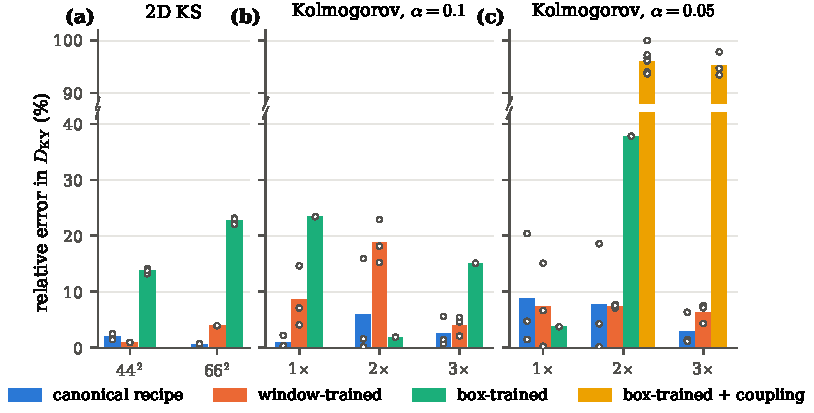
\includegraphics{figures/fig05_box_vs_window.pdf}
\caption{Relative error in $\DKY$ for four training recipes, on a linear
axis broken between $42\%$ and $88\%$; only the box-trained models with
added coupling land above the break. Bars are means over initial
conditions, dots individual initial conditions. Every window-trained and
canonical evaluation is below $25\%$, while box-trained models with
coupling miss by more than $90\%$. Box-trained: an $8\times8$-site
periodic box; with coupling: the exact Biot--Savart velocity (D2), a
learned regional scale (D3), or both box training and the exact velocity
(C9), all at $\alpha=0.05$; window-trained: the same architecture trained
on crops of a large domain; canonical: per-patch autoencoder with $c=6$
and long free rollouts. All evaluations use initial conditions
standardized with the training statistics, except the $\alpha=0.1$
box-trained $3\times$ value, for which only a raw-initial-condition
evaluation exists.}
\label{fig:box_vs_window}
\end{figure*}

\begin{figure*}[htbp]
\centering
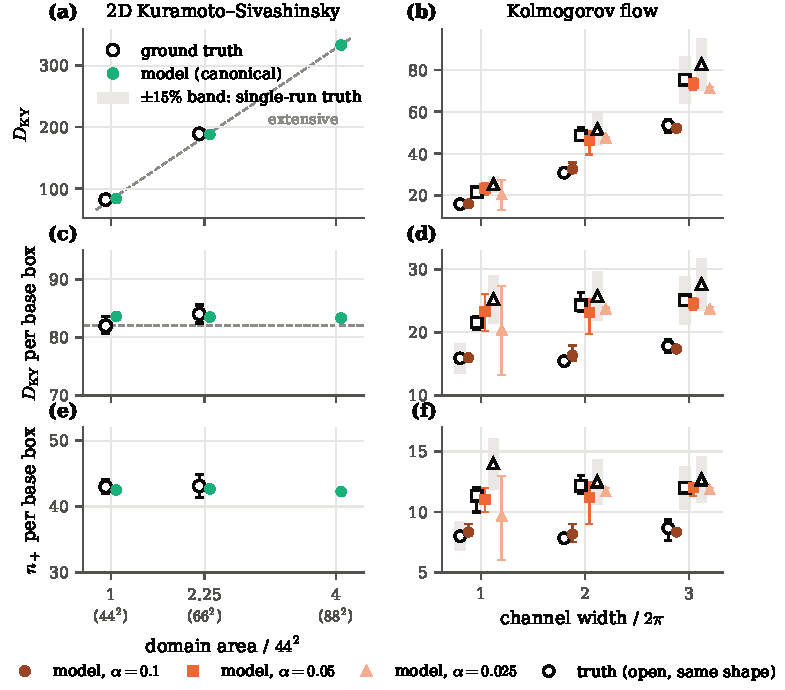
\includegraphics{figures/fig06_scaling.pdf}
\caption{Scaling of the dimension and of the number of unstable
directions with domain size. Rows: $\DKY$; $\DKY$ per base box ($44^2$
for 2D KS, $2\pi\times2\pi$ for Kolmogorov flow); number of positive
exponents $n_+$ per base box. Open markers: ground truth, with bars
spanning the runs where several exist and a shaded $\pm15\%$ band where a
size rests on one run (the run-to-run spread of Appendix~\ref{app:groundtruth});
filled markers: canonical models, with bars spanning initial
conditions. (a,c,e) 2D KS, where both sides of the box grow; the dashed
line is extensive scaling from the native truth. (b,d,f) Kolmogorov flow,
where the channel widens at fixed height; marker shape and lightness
give the drag. Both densities stay flat in 2D KS, for the truth and the
transferred model; in Kolmogorov flow the models track the truth at
$\alpha=0.1$ and $0.05$ and fall below it at $\alpha=0.025$.}
\label{fig:scaling}
\end{figure*}

\begin{figure*}[htbp]
\centering
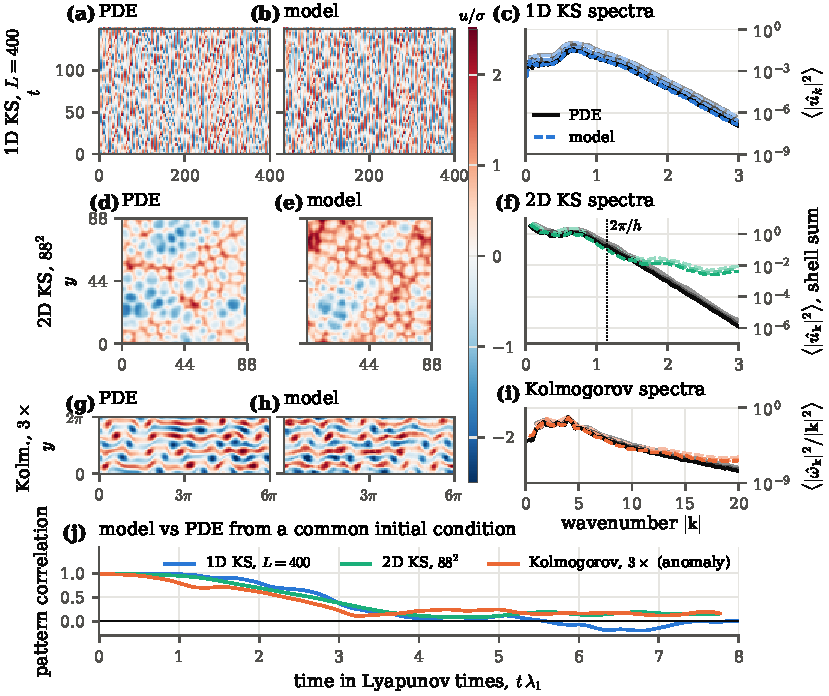
\includegraphics{figures/fig07_rollouts_spectra.pdf}
\caption{Free rollouts, energy spectra and pattern correlation after
transfer, one system per row; columns: PDE, transferred model from the
same encoded initial condition, time-averaged spectra against wavenumber
(solid: PDE; dashed: model; lighter lines: smaller domains). (a--c) 1D KS at $L=400$, four times the training size,
first 150 time units; spectra at $L=100$, $200$, $400$. (d--f) 2D KS at
$88^2$, four times the area of the base box, 35 time units after the
initial condition; spectra at $44^2$, $66^2$, $88^2$; the dotted line is
the patch wavenumber $2\pi/h$. (g--i) Kolmogorov flow at $\alpha=0.1$ and
$3\times$ (the main-text model), vorticity 40 time units after the initial
condition; kinetic-energy spectra at $1\times$, $2\times$, $3\times$.
Spectra: steps $100$--$999$ of a 1000-step rollout. (j) Spatial
correlation between model and PDE fields against time in Lyapunov times
$t\lambda_1$ (truth $\lambda_1$ at the largest size with a truth); for
Kolmogorov flow the PDE's mean vorticity profile in $y$, which is locked
to the forcing, is removed first. In all three systems the correlation
falls below $0.5$ after $2.3$--$2.9$ Lyapunov times while the spectra
stay on the PDE's: the models lose the trajectory, not the statistics.
In 2D it settles at $0.15$--$0.2$, a slowly varying large-scale component
shared over this window. The per-patch decoder leaves seams in 2D KS,
seen as excess energy beyond $2\pi/h$.}
\label{fig:rollouts}
\end{figure*}
